\chapter{Path Planning Algorithms}
\section{Algorithm Overview}

The output of the path generator should be a single trajectory that completely connects and covers all elements of the drawing.

This happens in three steps: First, the polygons that have to be filled are selected and the fill algorithm is seperately executed for each of the polygons with polygon specific settings. In a second step all of the drawing elements are connected by an open tour and tries to minimize the traveled distance by applying a traveling salesman heuristic. As last step, connections with limited curvature are generated to complete the trajectory.

Each of those steps will be discussed in detail in this section.
% here you set the main requirements connected, as short as possible, no sharp angles etc)
\section{Image Structure}

Derived from the requirements, three different elements were identified as part of drawing (also shown in \autoref{fig:elements_def}:

\begin{description}
\item[Polyline] A line consisting of $2$ to $n$ vertices
\item[Polygon] A closed line, consisting of $2$ to $n$ vertices, where the last segment is a closing one. So that vertex $v_{n+1}$ equals $v_0$.
\item[Filled Polygon] Defined in the same way as the polygon, except that the inner space should be filled by the generated trajectory. Another difference is that the filled polygon can also contain holes, which should not be covered and be excluded from the fill trajectory.
\end{description}

\begin{figure}
\centering
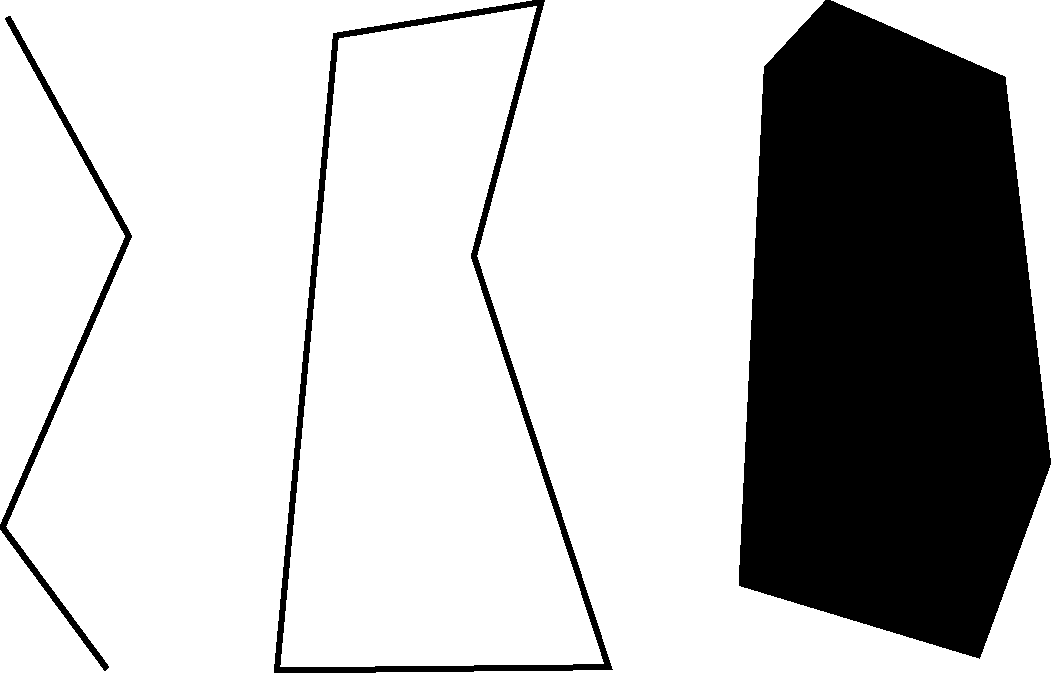
\includegraphics[width=0.6\textwidth]{images/path_planning/line_polygon_definition.pdf}
\caption{Polyline, polygon and filled polygon}
\label{fig:elements_def}
\end{figure}

% you discuss the lines, closed lines, filled polygons
% then you explain the structure that you work on elements separately and the connect them with TSP.
\section{Polygon Filling}

\subsection{Related Work}

Over time several surface coverage algorithms have been developed, and some distinctions can be made. 

Coverage algorithms exist for applications like autonomous vaccuum cleaners or autonomous lawn mowers, but also search and rescue robotic applications usually and they usually do not care if they visit the same spot twice. The target for those algorithms is rather to achieve complete coverage of an previously unknown terrain in sensible time. Usually, the complete surface coverage algorithms in are also connected with online map generation techniques \textit{SLAM}, whereas the path generation for the BeachBot should happen offline.

However, in agricultural applications some interesting algorithms have been found, which served as inspiration for the explorations presented in this thesis. Especially \citep{ROB:ROB20300}, who hinted at exploiting the straight skeleton algorithm to generate the inset polygons. An optimization strategy is employed to find the shortest trajectory through the field by repeatedly offsetting the remainding shape and traversing all possible ways off filling the shape. The algorithm is relatively computing intensive, what might be justified when using huge agricultural machines but what was not necessary for the goals of this thesis as the benefit of this optimization would be relatively small.

Another field where trajectories have to be generated is in \textit{Computer Aided Machining}. The process of removing layers of material from a block of metal is quite similar (though inverse, usually) to what is achieved in this thesis. Many publications deal with the problem of multi-axis milling machines which are far more complex and are also able to go over the machined surface without problem because they can lift the machnining head -- something that is not possible with the autonomous ground robot. 

One interesting publication in the CAM field is \cite{kao1998optimal} that presents a method to reduce gaps that are present when simply offsetting a polygon with spirals. The presented method could be a possible future improvement to the spiral fill algorithm of \autoref{sec:spiral_fill}.

The OpenCAM library has also been inspected...

	% all the algorithms go here
\subsection{Spiral Filling}

\subsubsection{Straight Skeleton}

To generate a spiral fill for the trajectory, we use the properties of the so called straight skeleton. The straight skeleton is defined as the topolgical skeleton of a polygon that is created by moving the edges inwards at a constant speed and observing the intersections of the vertices. It was first described by \citep{Aichholzer:jucs_1_12:a_novel_type_of}. 

During the creation of the straight skeleton, two events can happen: 

\begin{itemize}
\item Edge event: An edge shrinks to zero, making its neighboring edges adjacent now.
\item Split event: An edge is split, i.e., a reflex vertex runs into this edge, thus splitting the whole polygon. New adjacencies occur between the split edge and each of the two edges incident to the reflex vertex.
\end{itemize}
(cited from \citep{Aichholzer:jucs_1_12:a_novel_type_of}).

The straight skeleton is similar to the median axis of a polygon, but unlike the median axis it is not defined to have a constant distance to the polygon edges.

For the case of this thesis, the most interesting property of the straight skeleton is the ability to easily obtain inset polygons. The inset polygons are used to create a spiral fill for the polygons. The procedure is as follows:

\begin{itemize}
\item[(0)] The straight skeleton is generated
\item[(1)] The inset polygon is created
\item[(2)] If a split event has happened, then it is decided which polygon should be used to extend the current spiral (that is the one with the closer point to our current position). All the others are recursively filled in the same way. Additionally, a starting point to the spiral is passed, so that the beginning of the next spiral will be close to the current one. (The procedure restarts with the split polygon as input at (0)).
\item[(3)] The $n+1$ vertex of the inset polygon is appended to the current spiral
\item[(4)] An inset polygon is generated with inset length divided by number of vertices. Through dividing the inset length (which is predefined, usually as one rake width) by the number of vertices in the polygon, we make sure that one revolution of the spiral will travel only one rake distance.

\end{itemize}

\begin{algorithm}[H]
\begin{algorithmic}
\caption{Spiral Filling}\label{spiral_fill}

\Function{createSpiralFill}{Polygon p, Point startPoint}

\State $ss \gets \text{getStraightSkeleton}(p)$
\State $lOffset = RakeWidth/p.size()$
\If{$startPoint$} $currPoint \gets startPoint$ 
\Else ~$ currPoint \gets p[0]$ 
\EndIf
\While{$insetPolys.size() \geq 1$}
\If{$insetPolys.size() > 1$}
	\State $closestPoly = searchClosestPolygon(insetPolys, currPoint)$
	\ForAll{$\lbrace poly \in insetPolys | poly \not\in closestPoly\rbrace$}
		\State $createSpiralFill(poly)$
	\EndFor
	\State $ss \gets getStraightSkeleton(closestPoly)$
	\State $lOffset = RakeWidth/closestPoly.size()$
	\State $insetPolys \gets getOffsetPolygons(ss, lOffset)$
\EndIf
\State $index \gets findClosestIndex(currPoint, insetPolys[0])$
\State $currPoint \gets insetPolys[0].fromIndex(index + 1)$
\State $result.append(currPoint)$
\State $insetPolys \gets getOffsetPolygons(ss, lOffset)$
\EndWhile
\EndFunction

\end{algorithmic}
%\SetKwFunction{FRecurs}{FillPolygon}
%\Fn(){\FRecurs{some args}}{
% \KwData{Polygon P, Startpoint SP, RakeWidth}
% \KwResult{Single trajectory}
% CurrPoint = findNearestPoint(SP, P)\;
% CurrOffset = RakeWidth / P.numberVertices\;
% S = generateStraightSkeleton(P)\;
% O = generateOffsetPolygons(CurrOffset, S)\;
% \While{$O.numberOfPolygons > 0$}{
%  \If{$O.numberOfPolygons > 1$} {
%	P = findCloserPolygon(O, CurrPoint)\;
%  }
% }
% \caption{How to write algorithms}
\end{algorithm}

The algorithm is both displayed in pseudo code and graphically. 

\begin{figure}[htbp]
	\centering
    \begin{subfigure}[b]{0.45\textwidth}
    		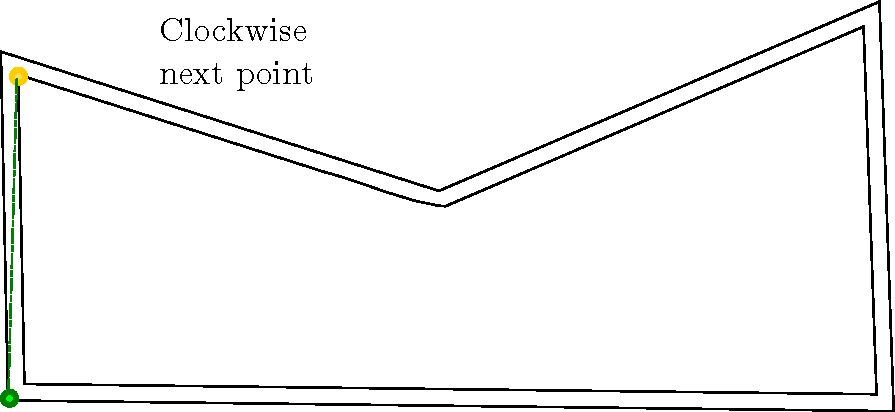
\includegraphics[width=\textwidth]{images/algorithms/spiral_fill/2.pdf}
		\caption{The first inset polygon and the first part of the spiral line}
    \end{subfigure}
    ~
    \begin{subfigure}[b]{0.45\textwidth}
    		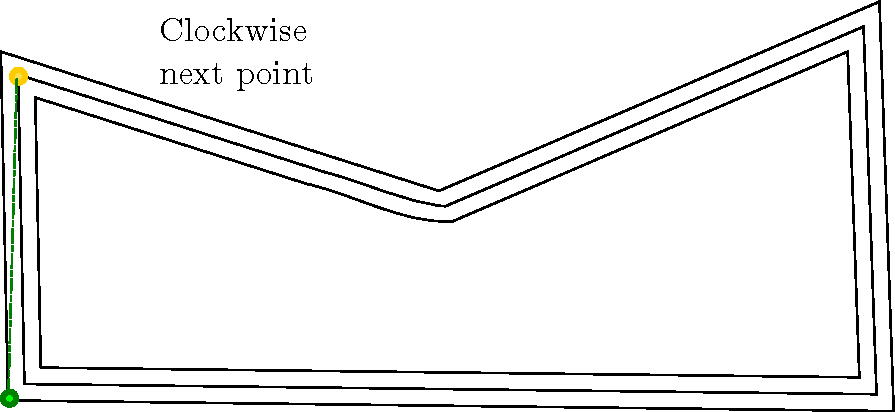
\includegraphics[width=\textwidth]{images/algorithms/spiral_fill/3.pdf}
    		\caption{Next inset polygon generated}
    \end{subfigure}\\
    \begin{subfigure}[b]{0.45\textwidth}
    		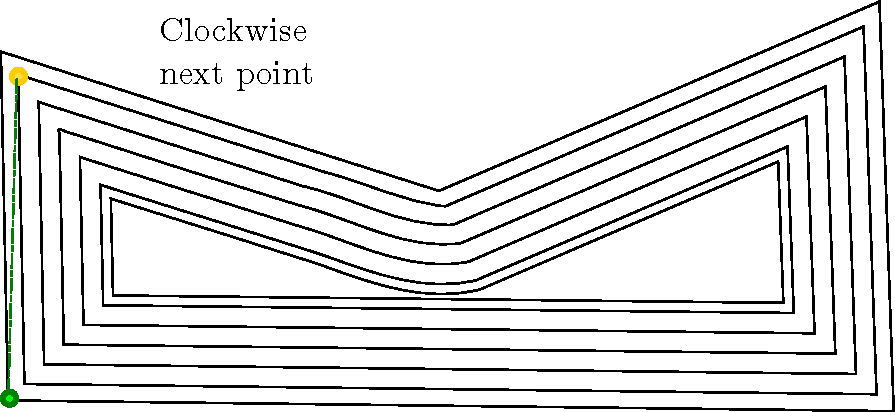
\includegraphics[width=\textwidth]{images/algorithms/spiral_fill/4.pdf}
    		\caption{The polygon right before the \textit{split} happens}
    \end{subfigure}~
    \begin{subfigure}[b]{0.45\textwidth}
    		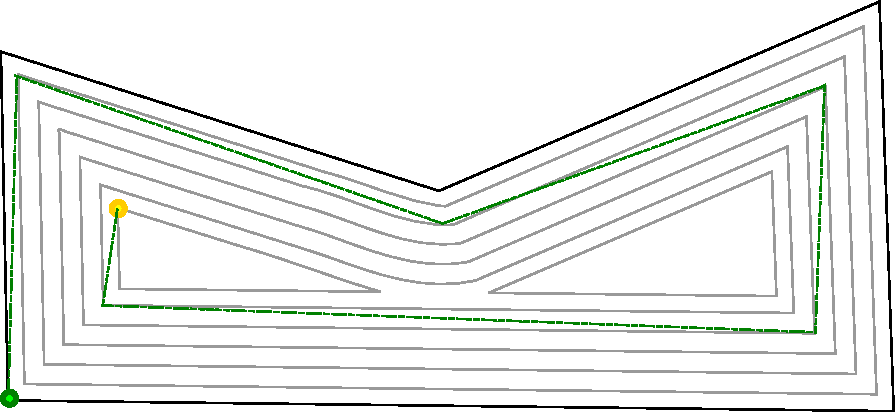
\includegraphics[width=\textwidth]{images/algorithms/spiral_fill/done.pdf}
    		\caption{After split, next polygon was found for continuing the current spiral}

    \end{subfigure}
        \begin{subfigure}[b]{0.45\textwidth}
    		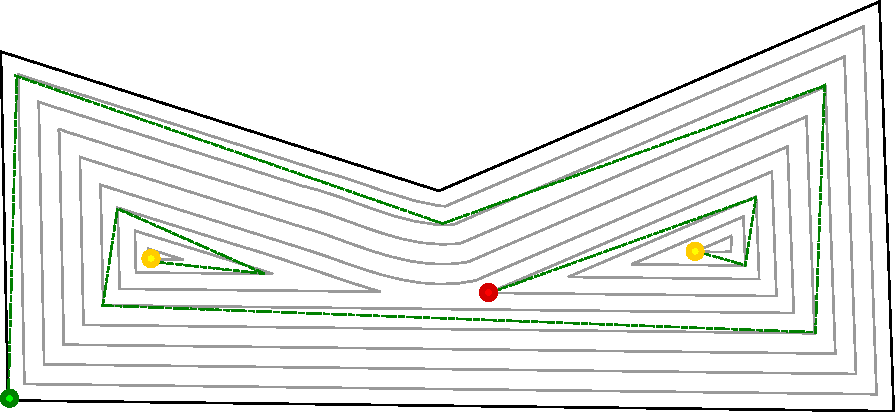
\includegraphics[width=\textwidth]{images/algorithms/spiral_fill/after_done_2.pdf}
    		\caption{Continuing spiral 1 and starting the second spiral. Note how the start point of the second spiral is the closest point to the endpoint of the first.} \label{splitevent}
    \end{subfigure}
\\
        \begin{subfigure}[b]{0.45\textwidth}
    		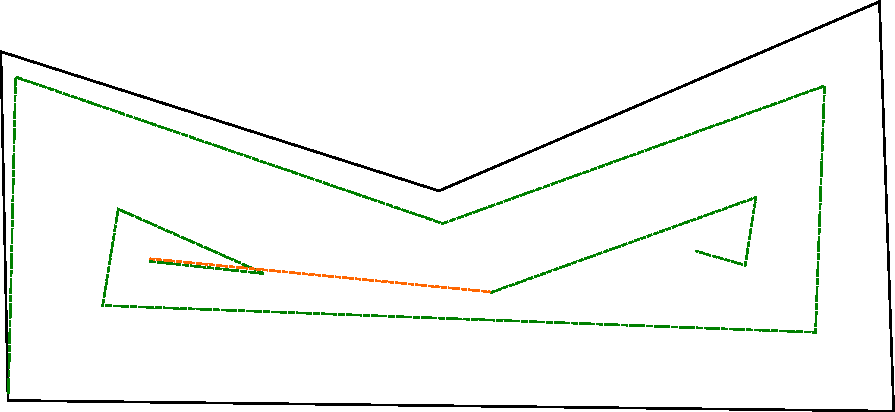
\includegraphics[width=\textwidth]{images/algorithms/spiral_fill/complete_done.pdf}
    		\caption{The completed spiral with all inset polygons removed.}
    \end{subfigure}
	\caption{Generating the fill spiral. Note that this is only an example for illustration purposes. Of course, the density of inset polygons for a real application is much higher.} \label{fig:insetting}
\end{figure}

\begin{figure}
\centering
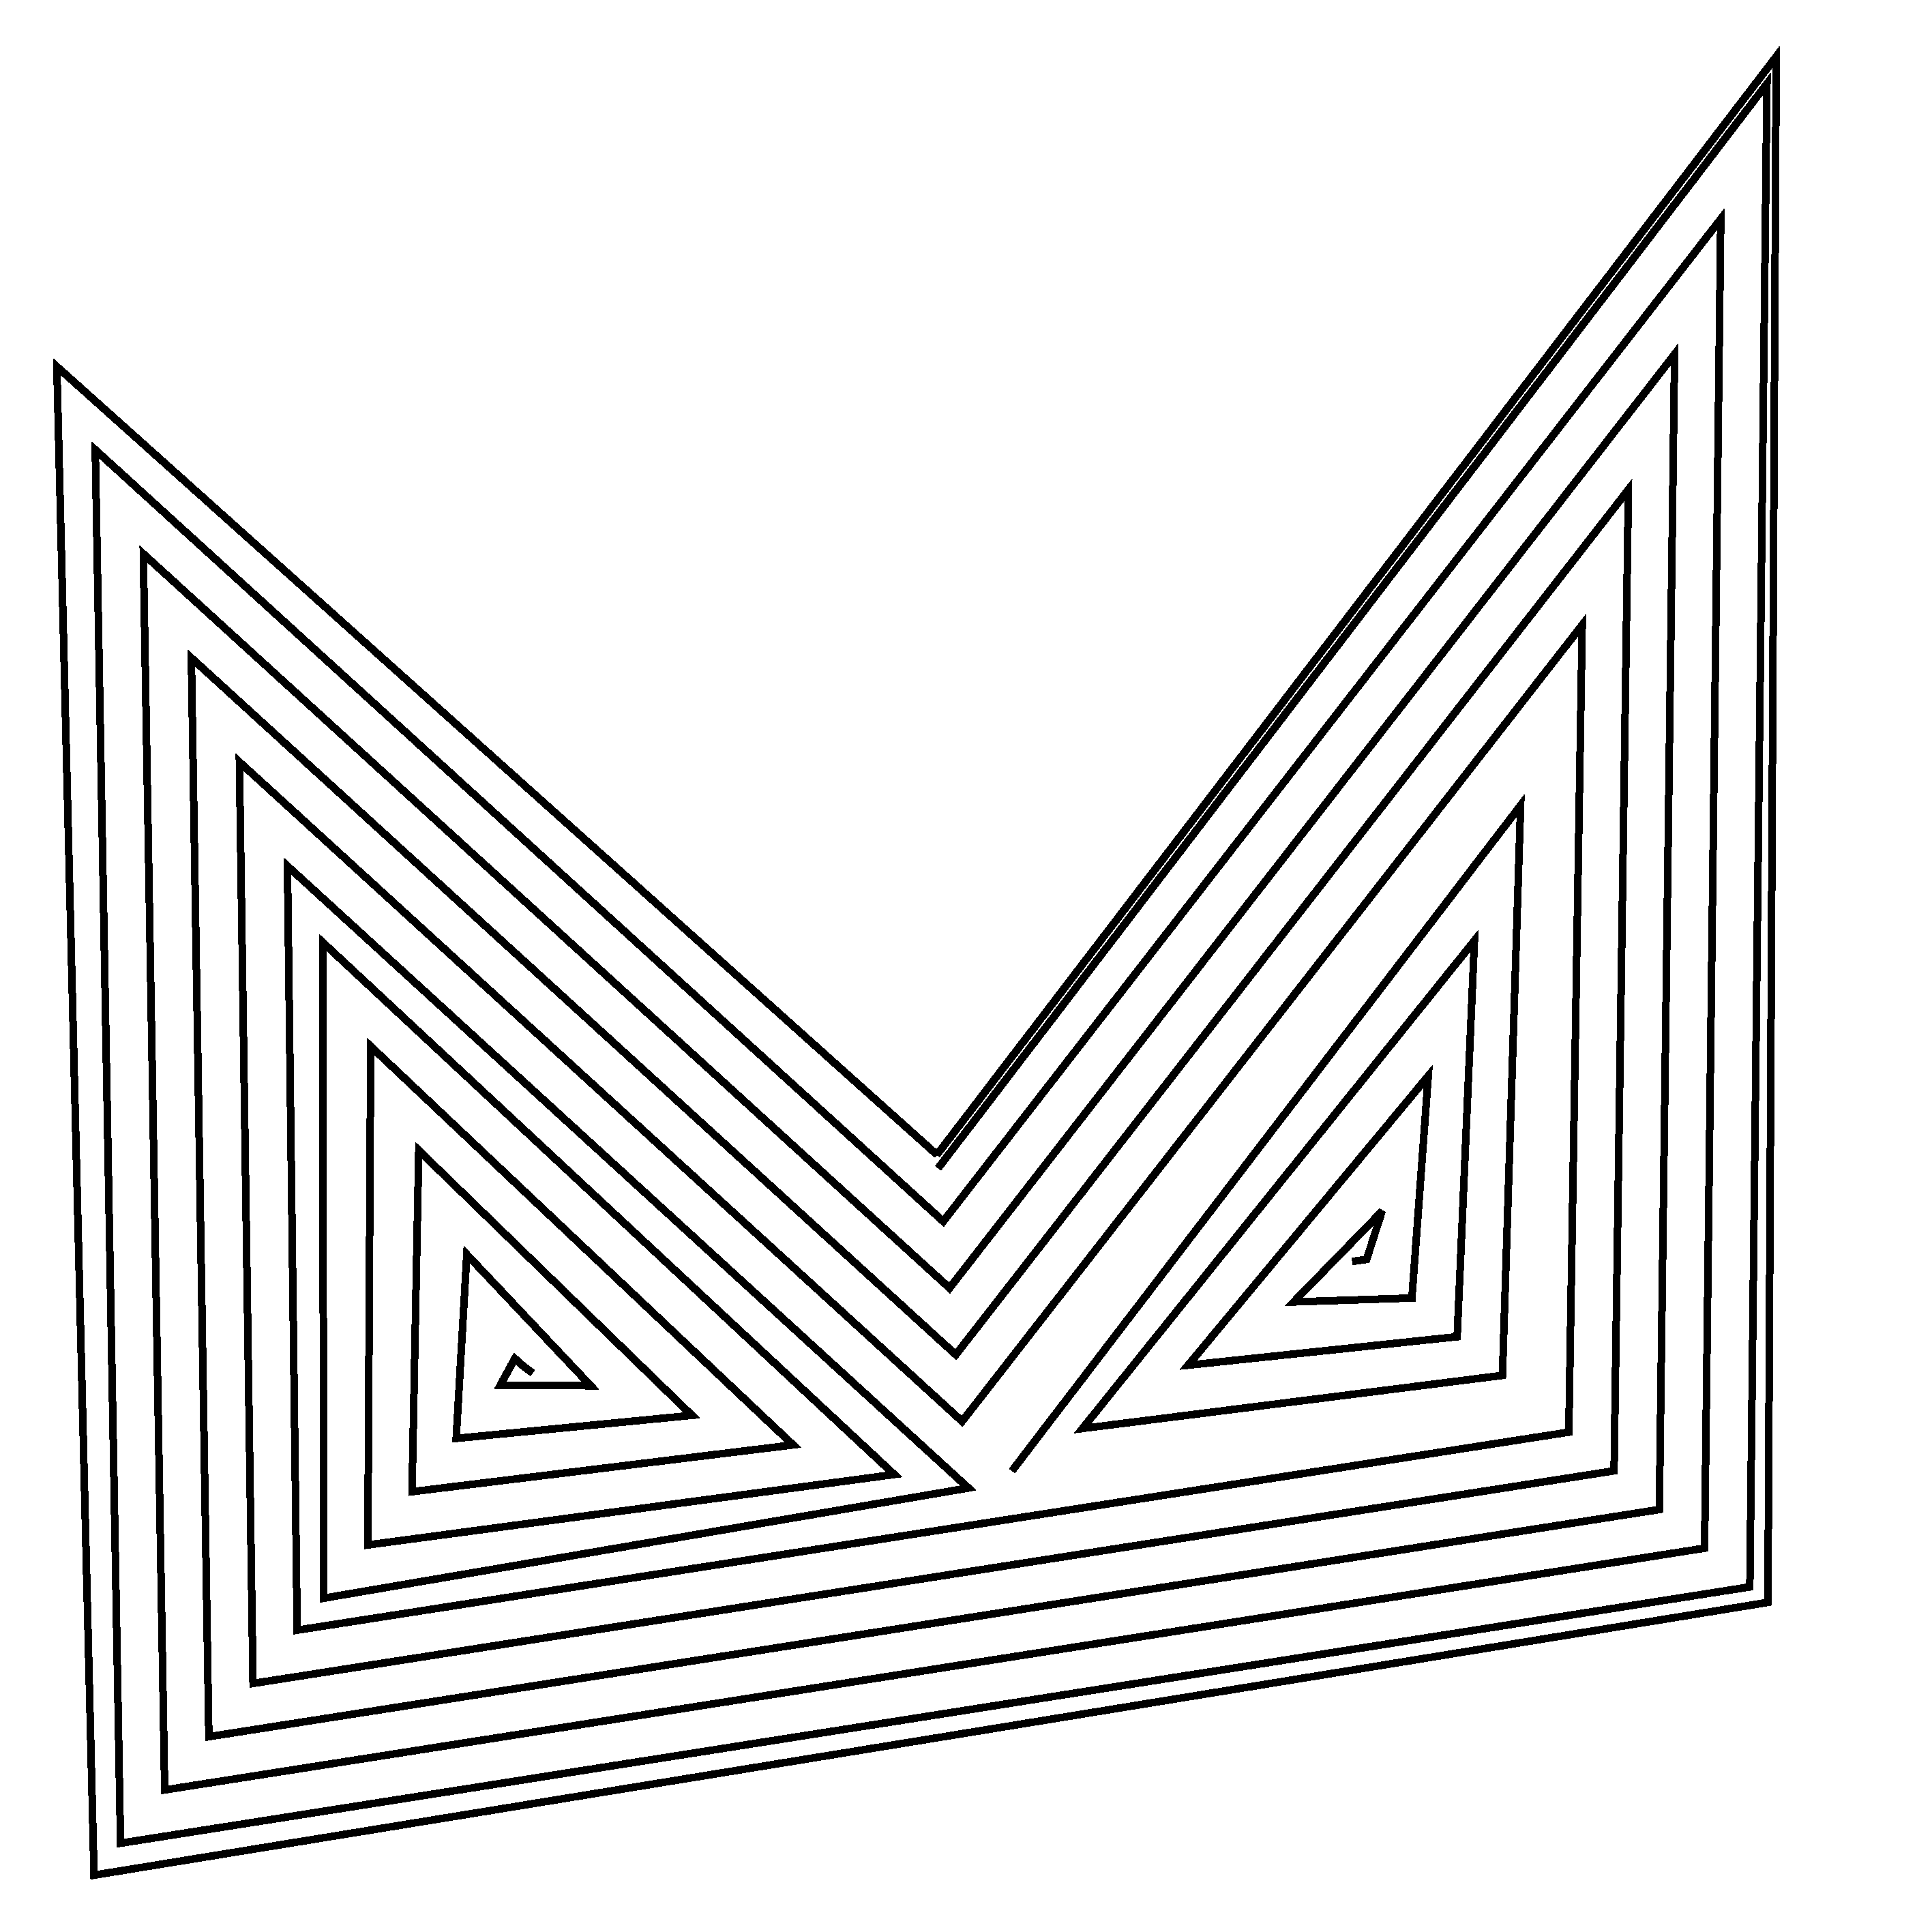
\includegraphics[width=0.6\textwidth]{images/algorithms/spiral_fill/spiral_real.pdf}
\caption{Generated spiral} \label{fig:gen_spiral}
\end{figure}

\subsection{Back and Forth Filling}

This fill method is quite straight forward: The polygon is filled by a number of lines that are parallel to each other and clipped at the polygon edges. The procedure takes an direction as input. 
First, a starting point is searched. If the inclination of the direction is bigger than 45°, then the leftmost vertex, whereas if the inclination is smaller, the bottommost vertex is selected.

Starting from the start point, lines are positioned with the specified direction and the polygon is tested for intersection. If two intersections for a given line are found, a line segment with those two points is added to the resulting trajectory.

This method works very well for convex polygons, but has drawbacks for non-convex polygons, since a non convex polygon can have more than two intersections for any given line. Therefore it requires the polygon to be decomposed into convex parts. This happens through optimal convex partitioning with the dynamic programming algorithm by Greene. The produced result is a set of convex polygons of maximum size, which is good for the purpose of filling the shape.


%et algorithm 
	% your algorithm. \subsubsection{Optimal Convex Partitioning} goes here without a special subsection for it

\section{Path Generation}
As already mentioned, to finally create a drawing all elements have to be connected by support trajectories where the rake is lifted. The supporting paths should have two properties: The total sum of all support paths should be as small as possible and the curvature of the connections should be limited.

As previously defined, a drawing consists of the three different types: Lines, polygons and filled polygons. Lines and polygons differ in the way they can be connected, as illustrated in \autoref{fig:connect}. A line can be entered or exited on both ends and is traversed in a previously unknown direction. A polygon however can be entered at any vertex, but can only be exited at the same so that the polygon is closed. Filled polygons work the same as the regular polygon in that sense, since the spiral and the back and forth filling create a polyline that is inserted into the filled polygon.

\begin{figure}
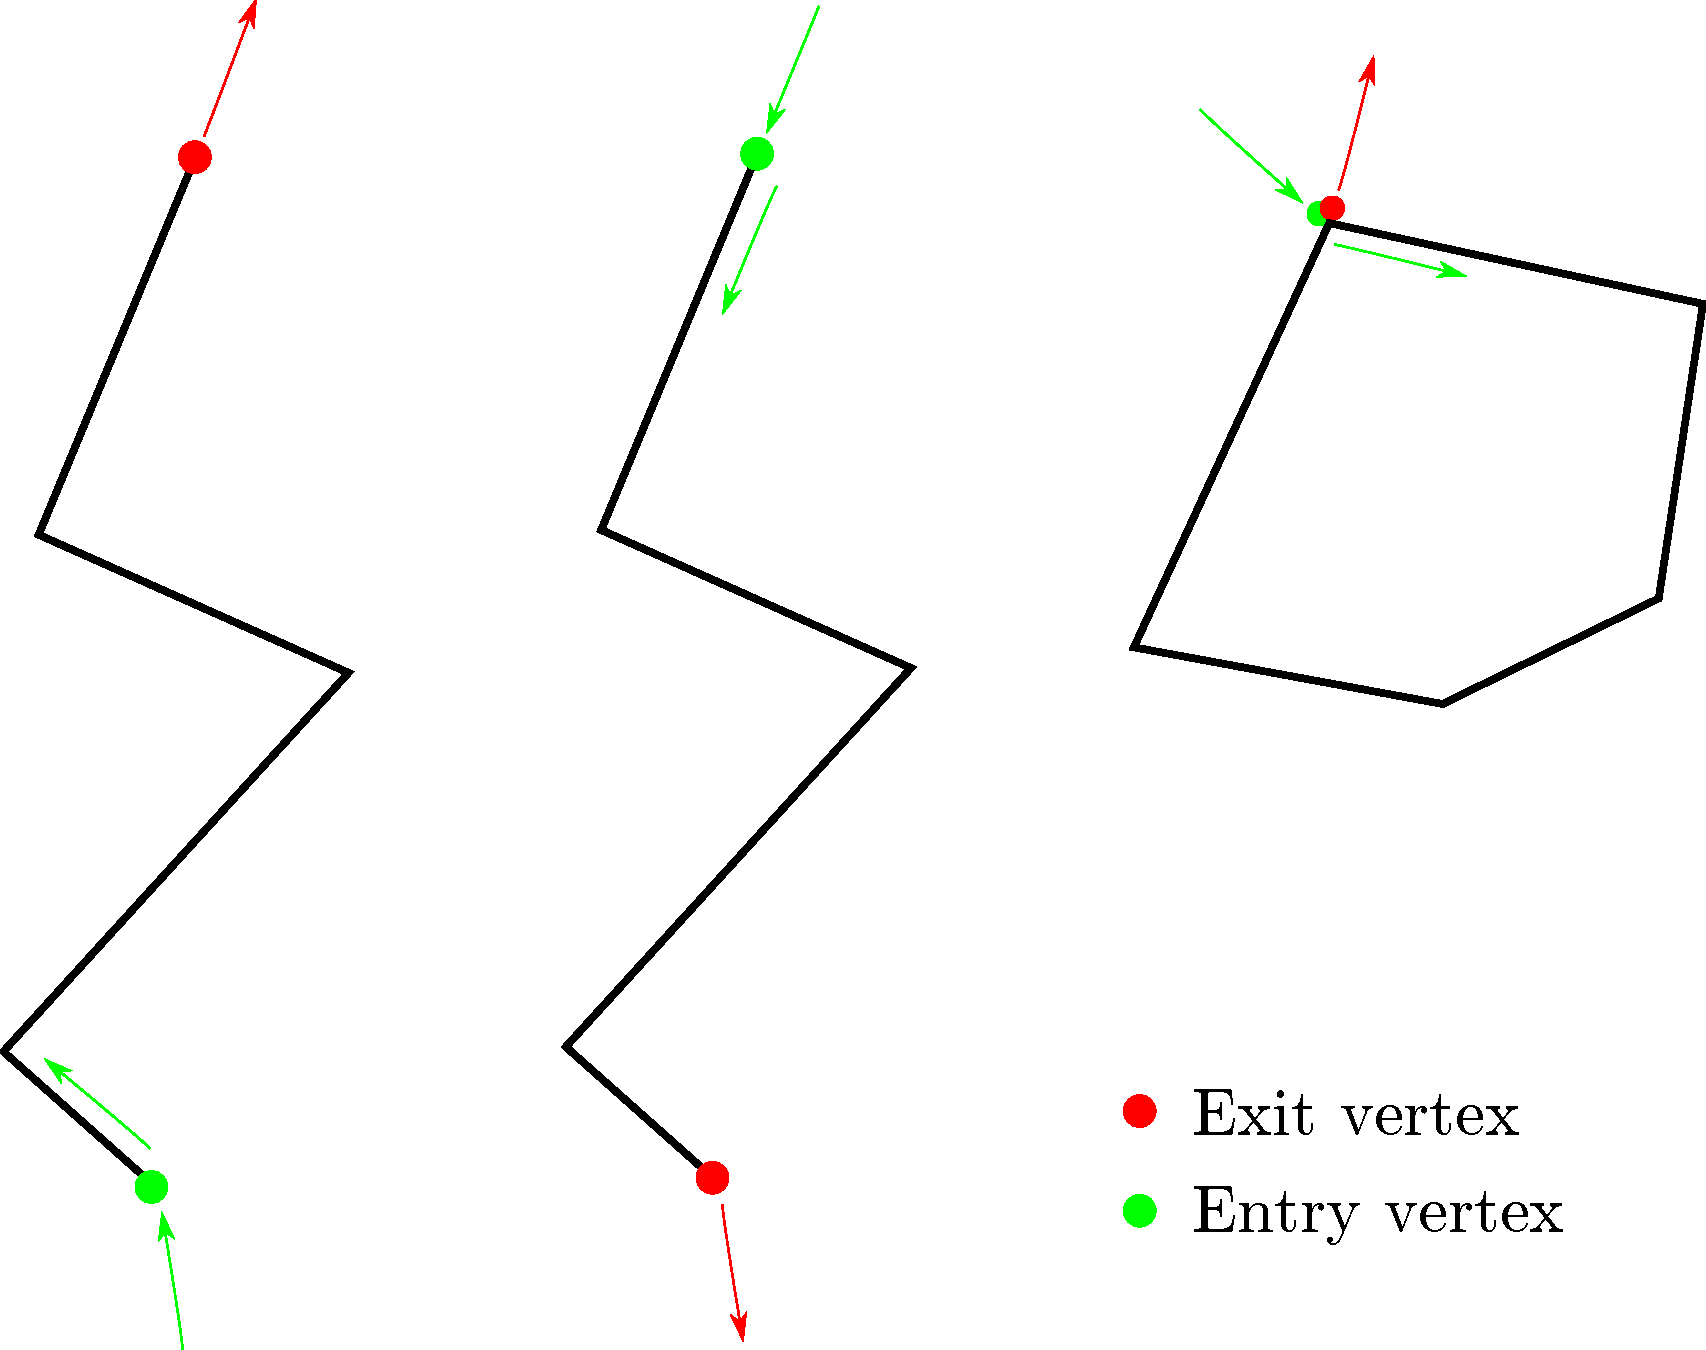
\includegraphics[width=0.8\textwidth]{images/path_planning/traversal.pdf}
\caption{Possible entry- and exit vertices and direction of traversal for polylines and polygons. Note that the polygon could also be traversed in clockwise direction.}
\end{figure}

\subsection{Traveling Salesman Problem}

The Traveling Salesman Problem (TSP) is the problem of finding the minimum-weight Hamiltonian Circuit in a weighted graph. A weighted graph is a graph where every edge between two vertices has a certain weight. The Hamiltonian Circuit is defined as a tour through the graph, that travels to every vertex exactly once. It is called salesman problem because in the historical context the vertices were cities and the salesman, seeking to minimize the distance traveled to visit all the cities in a given tour, would have liked to get a solution for this problem. However, one of the properties that make this problem hard is that it is NP-hard. If no heuristic is used, the amount of solutions that have to be searched in order to test all available possibilities is $n!$.

The TSP can be subcategorized in three categories: 

\begin{description}
\item[Symmetric] A TSP is symmetric if all distances between every node pair are symmetric (equal) in both directions from $A \leftrightarrows B$.
\item[Metric] In a metric traveling salesman problem, all distances conform to the triangle inequality $c \leq a + b$ which is, for example, true if all distances are calculated using the euclidean distance formula between two points: $\overline{AB} = \sqrt{(x_1 -x_2)^2 + (y_1 - y_2)^2}$ but also for the so called Manhattan distance which is defined as $\overline{AB_M} = |x_1-x_2| + |y_1 - y_2|$.
\item[Asymmetric] If the weights are different from $A \rightarrow B$ than from $B \rightarrow A$ then the TSP is assymetric. Of course, the triangle inequality cannot be fulfilled anymore.
\end{description}

The simplest heuristic to the TSP is the nearest neighbour search. From a given startpoint the nearest, unvisited vertex is searched and connected. This is done until no more unvisited elements exist. Positive about the nearest neighbour approach is that the complexity is only growing linear to the search size. However, the obtained solutions are often of unsatisfying quality.

Another popular heuristic is the branch and bound method. It works by splitting the set of possible solution into two halves and calculating a upper and lower bound for both. If the upper bound of the first is lower than the lower bound of the second, the second is discarded. During the course of this thesis a variant of the depth-first branch and bound search was implemented. First, the graph was traversed until a tour was completed. Afterwards, another tour (in order) was recursively started. As soon as the traveled distance of the entire tour in that branch got higher than the current minimum tour, the branch is discared. While this already reduces the search space, the effect becomes relatively small on larger problems (e.g. the first 6 out of 15 nodes might only seldomly span a tour which distance is higher than the current minimum, and it gets only worse).  It must be said, that the implementation was not very mature, and it actually produces an optimal tour in the current implementation, which is not desired in a heuristic. With more level-wise bounds it could have been a lot more efficient. 

The final solution to the minimum connection problem was to use a state of the art TSP solver\cite{helsgaun2000effective}, which employs the Lin-Kernhighan-Heuristic\cite{kernighan1970efficient} (LKH) to approximately solve the Traveling Salesman Problem. It is, unlike many other TSP solver implementations that require the triangle inequality to hold, also well suited to solve assymetric problems.
% general definition
% all three methods we tried, including LKH
\subsection{Adaptation of Traveling Salesman Problem for the Algorithm}

To find a suited tour with the generic LKH solver, the correct weights for the graph have to be specified. This happens in logical steps:

\begin{itemize}
\item On polylines, all vertices that are not the first or last node are removed, since they can never be accessed without entering at either the first or last node 
\item Polygons can be entered at any node. However, once entered, the polygon cannot be exited at any location but must be traversed completely. To enforce this, the weights on the polygon edges are set to be zero for the next vertex in clockwise direction and infinity for all other nodes of the polygon.
\item Every node is only visited once. This leads to problems in polygons, where the tour should be closed. There are two possible solutions: Double cities or weight shifting. Since the double cities approach is doubling the number of cities it is clearly the less optimal approach. Because it is known that entering at node $n$ will result in the visitor ending up at node $n-1$ (all edges are zero), using the weight shifting method, the outgoing weights of the polygon at node $n$ are shifted to node $n-1$. Thereby, the elementwise symmetry is restored and a optimal solution can be found with a generic TSP solver. In a post processing step, the polygon is closed again.
\item All other edge weights are the euclidean distances between the vertex pair
\end{itemize}

A regular TSP tour is closed. This implies that a regular tour has a tendency to go back to the starting point after diverging into another direction at the beginning. The solution that was found is to enforce a defined start point to be inserted. The outgoing weights of the start point are either euclidean distances or defined to be the same to every node in the graph. If they are euclidean, chances are very high that the starting line is the nearest neighbour. If the outgoing weights are all defined to be $1$ the LKH can find the best suited start point on it's own because the startpoint will not induce any preference for any of the nodes.

The ingoing weights for the startpoint are chosen to be equal for all nodes. Thus, the TSP will never optimize towards traveling back to the start point.

\section{Smooth Line Connections}

While not required by the robot kinematics of the BeachBot (which can turn on the spot), generating smooth connections is beneficial to the path converter that translates the generated rake path into a robot path that is drivable by the bot. If the curvature at a given point in the connection is too high, it is not possible for the path converter to find a converging solution which makes tedious manual work needed to adjust the curvature of the connections until the converter is able to find a solution. The rounded connections would also create a nice visual effect for spectators.

Ideally a way would have to be found that limits the curvature of the connection path.

Curvature is defined as the inverse of the radius of the circle that the tangent produces at any given point in the curve. For a two dimensional curve, the curvature $\kappa$ is defined as 
$$\kappa = \frac{|x'y''-y'x''|}{(x'^2+y'^2)^{3/2}}$$


\subsubsection{Beziér Splines}

A first approach to generate more curved connections was to use Beziér splines.
The start- and endpoint of the beziér spline is trivially found as the start- and endpoint of the connection. As first solution, we used beziér splines of 3rd order. Beziér splines of 3rd order only yield 2 control points, which can, by moving them along the desired tangent, easily be used to create a connection that is smooth in the start and endpoint. However, the curvature for the complete curve can not be set because the two control points offer to few degrees of freedom. A beziér curve of 5th degree (quintic) has enough DOF to constrain the connection in terms of curvature.

The quintic Beziér curve consists of 6 control points $P_0 ... P_5$ that define the shape of the curve. $P_0$ and $P_5$ are trivially chosen because they coincide with the start- respectively the endpoint of the curves that should be connected. $P_1$ and $P_4$ are also easy to choose as they have to lie on the tangents of the curves that should be connected. $P_2$ and $P_3$ on the other hand are more difficult to obtain. Even after an extensive search through available literature it remained unclear if an analytical solution to this problem can be found or not, since the equation for curvature is getting quite complicated if expanded. In \cite{doi:10.1137/1.9781611971521.ch5} three approaches to generate beziér splines with monotone curvature are discussed. \cite{choi2010piecewise} uses piecewise 3rd degree bezier curves to create a curvature and corridor constrained trajectory.  [to be expanded]

\subsubsection{Spiro Splines}

Spiro splines, introduced by \cite{levien2009spiral} are a different approach to designing fair curves, initially for the purpose of designing fonts. They have several properties which make them well-suited for the task at hand:

They offer 4 different control points to control the shape of the curve. In contrast to beziér curves, spiro spline control points are always passed by the generated curve, whereas the bezier curve only goes through the first and last control point. The 4 different control points, denoted by a single character, of spiro splines are:

\begin{itemize}
\item[\texttt{v}] Corner point
\item[\texttt{c}] A $G^2$ continous constraint. The curvature  on the left side is the same as on the right side ($\kappa_l = \kappa_r$).
\item[\texttt{o}] Similiar to \texttt{c}, a $G^4$ continous constraint. Not only $\kappa_l = \kappa_r$ is true, but also the first and second derivative of the curvature is constrained ($\kappa_l' = \kappa_r'$, $\kappa_l'' = \kappa_r''$).
\item[\texttt{[}] A straight-to-curved control point that acts like a tangent constraint in this case.
\item[\texttt{]}] A curved-to-straight control point that also acts like a tangent constraint here.
\end{itemize}

The author, Raph Levien, has licensed his implementation \footnote{libspiro: \url{http://www.levien.com/spiro/} } of spiro splines under the GPLv2, which makes it possible to be used by this thesis. The implementation is capable of being used for realtime editing. That guarantees that the curve generation would not be the bottleneck of the application in terms of time consumption. The output of the library is a set of Beziér curves which are easier to handle in regular graphics programs.

\paragraph{Heuristic for Setting the Control Points}

To find suitable locations for the spiro spline control points, a heuristic was used.

All connection constraints can be expressed by 5 variables: Connection length ($d$), tangents with angles $\alpha$ and $\beta$ and the curvature limit $\kappa$, as shown in \autoref{fig:connection_vars}. For the calculation of the control points, the difference between the two angles was defined as $\delta = \alpha - \beta$. It equals the angle between the two tangent vectors. 

Finding the first 4 points of the curve is straightforward: The first control point is a corner point at the endpoint of the first element. The second point is a straight-to-curve point, that is positioned an infinitesimally small distance in the direction of the tangent from the first point. This constrains the \enquote{outgoing} tangent. Vice versa, the same control points are set at the end of the curve, where the element that is connected with begins. Thus both tangent constrains are fullfilled. Because the spiros do not offer a direct way of setting the maximum and minimum curvatures, zero to two more control points have to be added. The curvature can be limited by positioning a $G^2$ control point at distance $2 * R$ from the start- and endpoint. This limits the curvature to the left and to the right to be the same. Since the highest curvature between the startpoint and the $G^2$ point would be a circular arc with radius $R$ this limits the curvature to $\kappa = 1/R$, as long as both $G^2$ points are keeping a distance of $2*R$ as well.

The heuristic differentiates 3 cases:

If the both tangent vectors $\alpha$ and $\beta$ have a similar direction and the circle that is described by them and $d$ has a radius that is in the range of $R < r < 2*R$ then no intermediate $G^2$ points are set because the connection will already be smooth and optimal.

Otherwise, the $G^2$ points are set by elongating the tangent vector to $2*R$ and rotating it by $0.5 * \alpha$. This is done to reduce the size of the resulting curve, which is demonstrated in .. Fig ...

As discussed, the two $G^2$ points, called $c_1$ and $c_2$ are closer than $2 * R$ to each other, the positions have to be recalculated. This happens by rotating the $c_1$ and $c_2$ points gradually in different direction until positions are found that conform to the distance constraint. By rotating both points about the same angle, a symmetry is kept.

If the distance $d$ is smaller than 

\begin{figure}

\usetikzlibrary{calc}

\definecolor{cb3b3b3}{RGB}{179,179,179}
\definecolor{ccccccc}{RGB}{204,204,204}
\definecolor{cffffff}{RGB}{255,255,255}

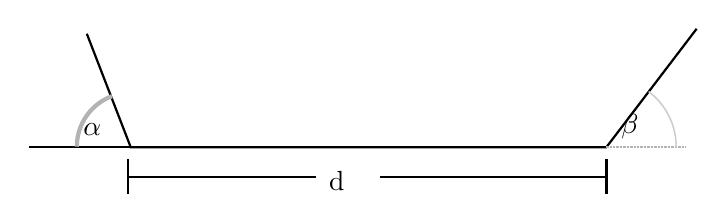
\begin{tikzpicture}[y=0.80pt,x=0.80pt,yscale=-1, inner sep=0pt, outer sep=0pt]
\centering
  \path[draw=black,line join=miter,line cap=butt,line width=0.800pt]
    (96.0814,121.3474) -- (115.9166,172.6195) -- (330.7355,172.6195) --
    (371.5287,119.1019);
  \path[draw=black,line join=miter,line cap=butt,line width=0.800pt]
    (115.9129,172.6241) -- (69.8665,172.6241);
  \path[draw=cb3b3b3,dash pattern=on 0.34pt off 0.17pt,line join=miter,line
    cap=butt,miter limit=4.00,dash phase=0.201pt,line width=0.800pt]
    (330.6888,172.6195) -- (366.5496,172.6195);
  \path[cm={{1.45393,0.0,0.0,1.45393,(-471.01666,-377.22731)}},draw=ccccccc,miter
    limit=4.00,line width=0.550pt] (564.5997,360.8878)arc(-52.961:0.593:21.466);
  \path[cm={{0.52395,0.0,0.0,0.52395,(41.81533,-25.47312)}},draw=cb3b3b3,miter
    limit=4.00,dash phase=0.960pt,line width=1.527pt]
    (94.9543,377.5908)arc(179.987:249.624:46.467);
  \path[fill=black,line width=0.800pt] (94.482018,167.26112) node[above right]
    (text4046) {$\alpha$};
  \path[fill=black] (337.53653,168.90082) node[above right] (text4046-2)
    {$\beta$};
  \path[draw=black,line join=miter,line cap=butt,line width=0.800pt]
    (114.8543,177.9195) -- (114.8543,193.7975);
  \path[draw=black,line join=miter,line cap=butt,line width=0.800pt]
    (114.8543,186.1205) -- (330.7957,186.1205);
  \path[draw=black,line join=miter,line cap=butt,line width=0.800pt]
    (330.7957,177.9195) -- (330.7957,193.7975);
  \path[fill=cffffff,line width=0.800pt,rounded corners=0.0000cm]
    (199.5575,177.5072) rectangle (228.2820,192.5707);
  \path[fill=black,line width=0.800pt] (205.50471,192.37236) node[above right]
    (text4081) {d};
\end{tikzpicture}
\caption{Variables for the connection between two elements}
\label{fig:connections_vars}
\end{figure}
